\subsection{The detectors}
\begin{frame}{The two detectors - SiD and ILD}
\ilclogo
\begin{block}{}
The ILC has only one interaction point (IP)!\\
The two detectors can be swapped in the so-called \textbf{push-pull-system}.
\end{block}

\begin{columns}
\begin{column}{0.5\textwidth}
\begin{center}
\visible<2->{\alert{SiD - Silicon Detector}
\begin{itemize}
\item Height: $\sim$\SI{14}{\metre}, length:  $\sim$\SI{11}{\metre}
\item Weight: $\sim$\SI{10100}{\tonne}
\item Supercond. solenoid field: \SI{5}{\tesla}
\item Full silicon tracker
\end{itemize}
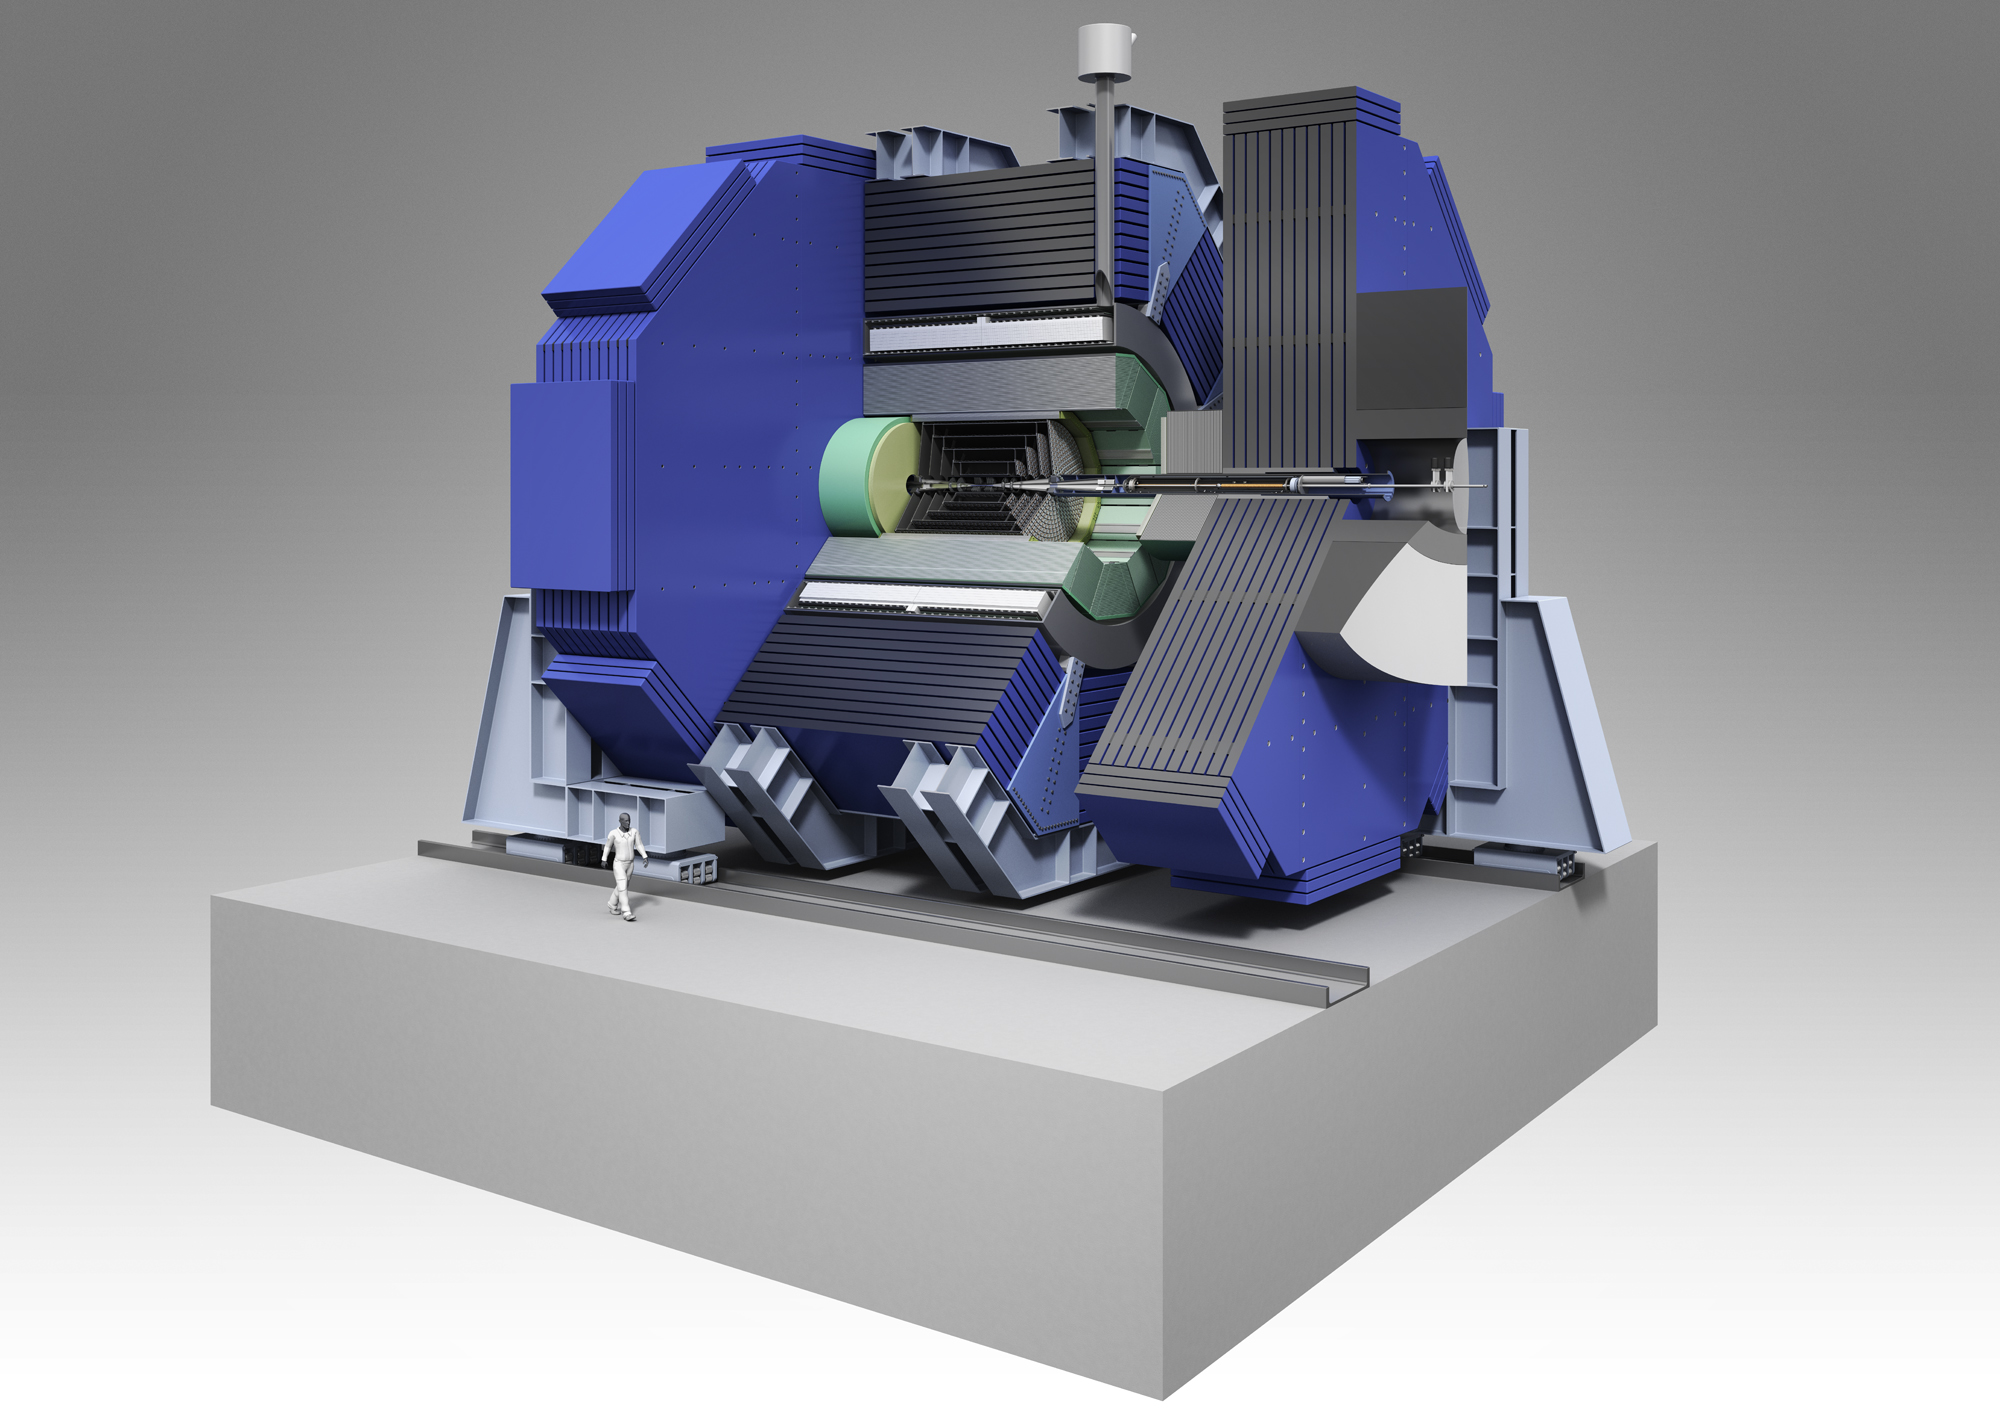
\includegraphics[width=0.45\textwidth]{figures/SiDmodel.jpg}\\
}
\end{center}
\end{column}
\begin{column}{0.5\textwidth}
\begin{center}
\visible<2->{\alert{ILD - International Large Detector}
\begin{itemize}
\item Height: $\sim$\SI{16}{\metre}, length:  $\sim$\SI{14}{\metre}
\item Weight: $\sim$\SI{14000}{\tonne}
\item Supercond. solenoid field: \SI{3.5}{\tesla}
\item TPC
\end{itemize}
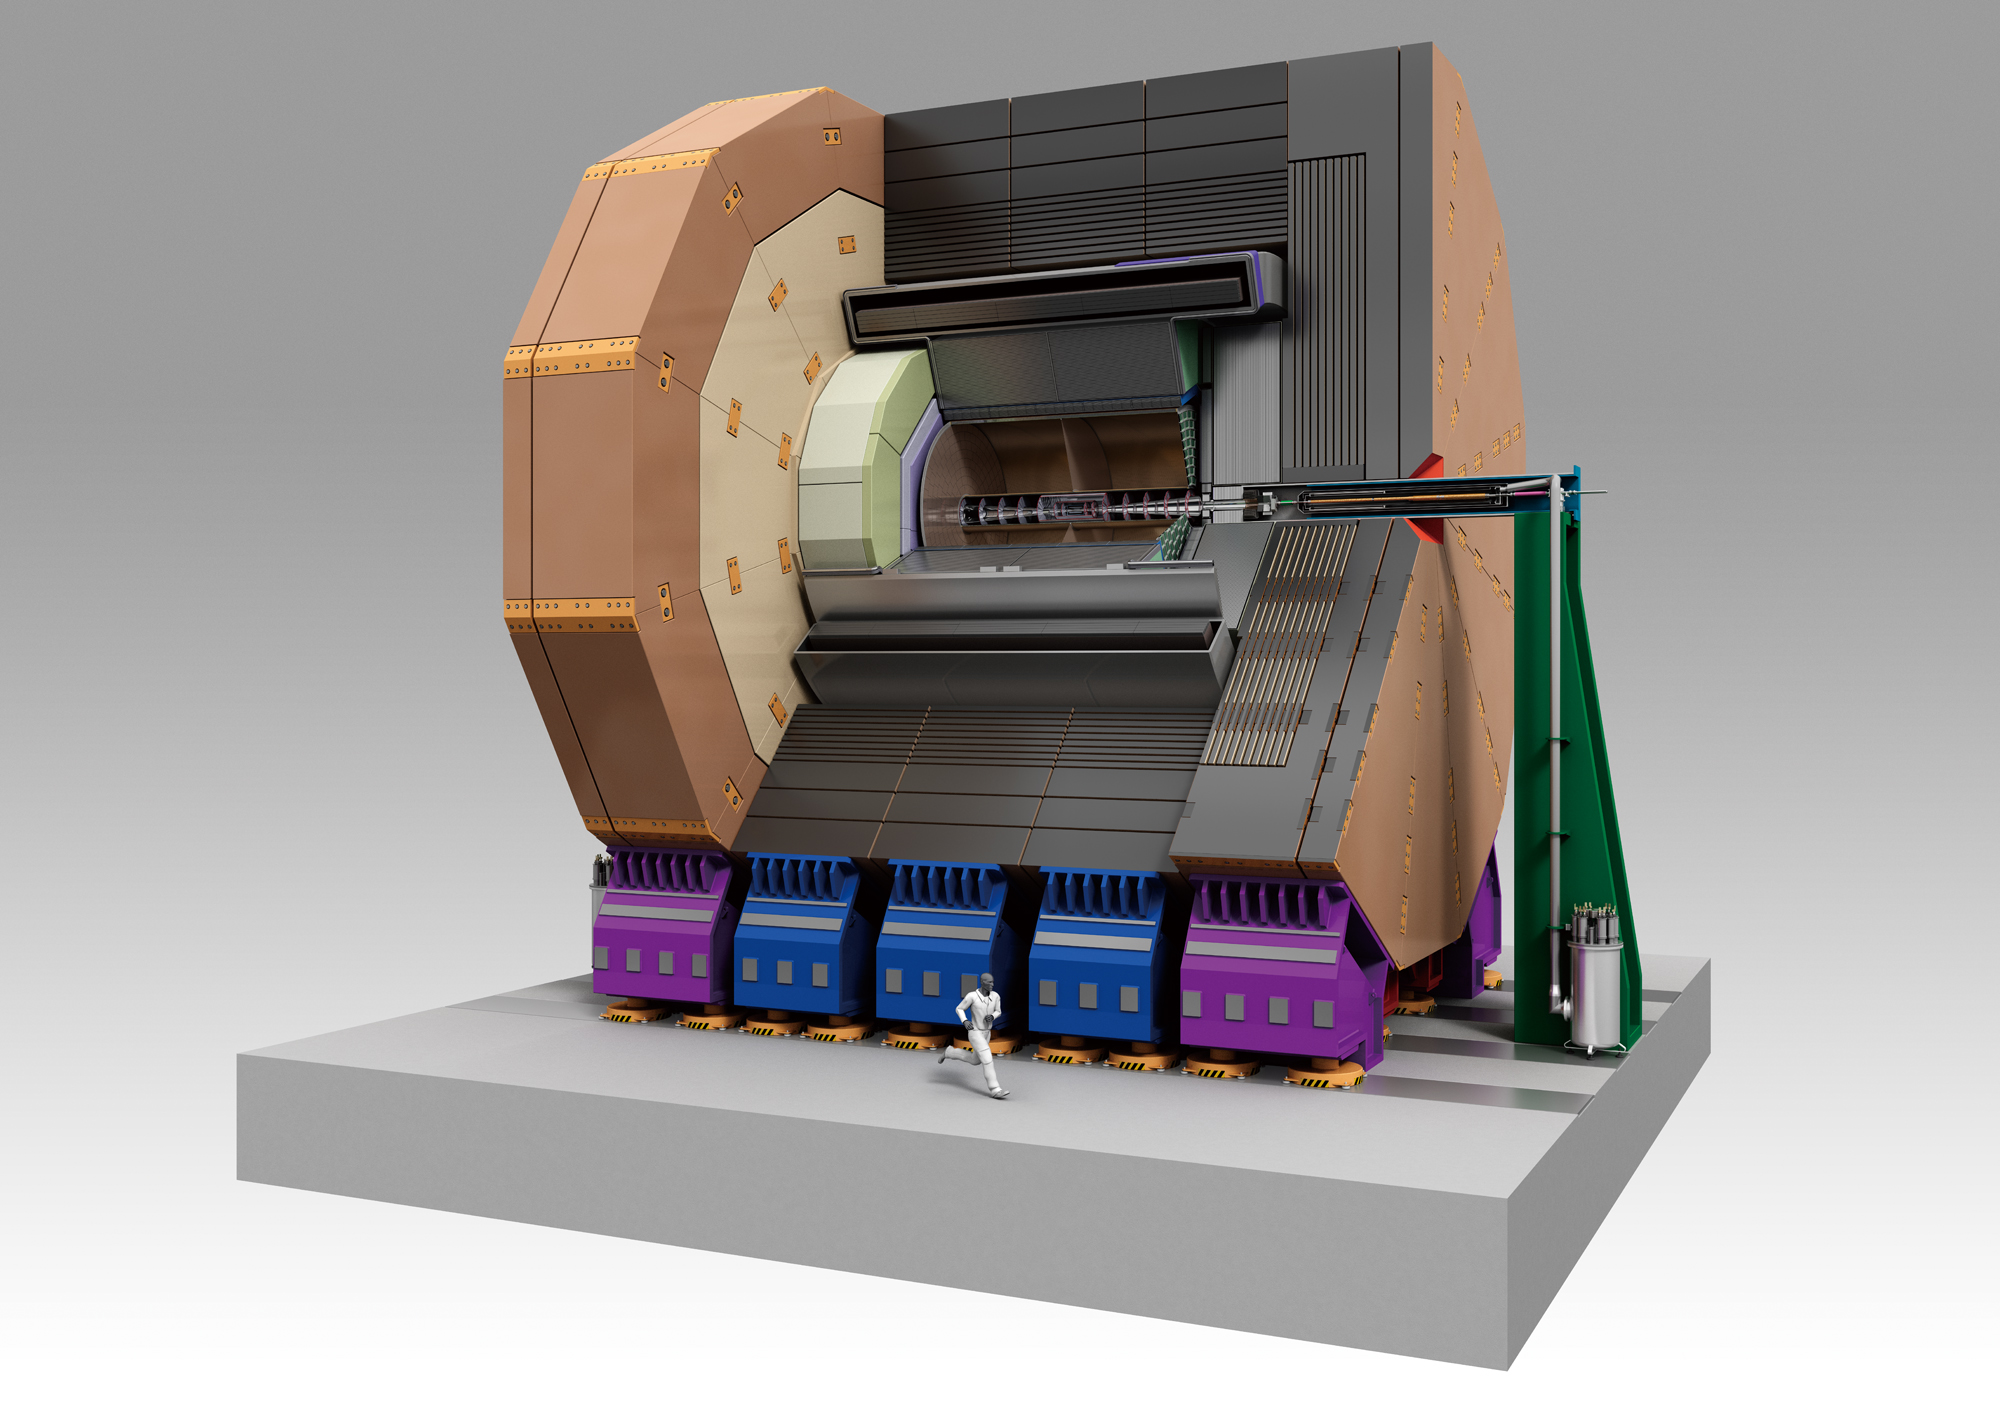
\includegraphics[width=0.45\textwidth]{figures/ILDmodel.jpg}
}
\end{center}
\end{column}
\end{columns}

\end{frame}

